\section{Netzarchitektur}
\label{spektrale_netzarchitektur}

Die Architektur eines neuronalen Netzes auf Graphen mit spektralen Faltungen verhält sich durch die ähnliche Formulierung einer Faltungs- und einer Poo\-ling\-sch\-icht analog zu der Netzarchitektur klassischer \glspl{CNN}.
Dabei werden wie gewohnt mehrere Faltungsschichten mit stetig erhöhter Merkmalsausbreitung aneinander gereiht und an einigen Stellen über Poolingschichten getrennt, die die Anzahl der zu betrachtenden Knoten sukzessive reduzieren.
Im Anschluss darauf finden sich im Allgemeinen zwei bis drei vollverbundene Schichten, die die Merkmalsgröße dann schlussendlich auf die gewünschte Ausgabegröße reduzieren~\cite{Nielsen}.
Die mehrmalige Verkettung von Faltungsschichten sorgt dafür, dass auch bei einer relativ kleinen Faltung über die lokale Nachbarschaft eines jeden Knoten Merkmale weit entfernterer Knoten gewonnen werden können.

\glspl{CNN} auf Bildern erfordern dabei in einer analogen Netzarchitektur eine feste Eingabegröße.
Dafür werden die Bildermengen in der Regel insofern skaliert und zugeschnitten, dass diese alle die gleiche Bildgröße besitzen (\zB{} $224 \times 224$)~\cite{spp}.
Es erscheint jedoch schwierig, eine Menge von Graphen soweit anzupassen, dass diese alle die gleiche Anzahl an Knoten aufweisen.
So ist es zwar vorstellbar, zusätzliche \enquote{Fake}-Knoten zu jedem Graphen hinzufügen, damit diese alle eine feste Anzahl an Knoten aufweisen.
Neben dem erhöhtem Speicheraufwand ist dieser Ansatz jedoch insbesondere nicht geeignet für unbekannte Graphen, die in das Netz eingespeist werden.
So können diese \evtl{} eine größere Anzahl als die zuvor festgelegte Größe aufweisen.
Ebenso liefert uns der Prozess der Graphvergröberung eine stets unterschiedliche Repräsentation eines Graphen, die wohlmöglich bereits eine größere Menge an \enquote{Fake}-Knoten hinzufügt und dabei die festgelegte Knotengröße der Graphen überschreitet.
Es ist weiterhin schwierig, einen Graphen auf eine feste Größe zuzuschneiden.
So ist es insbesondere nicht ersichtlich, welche Knoten aus einem Graphen entfernt oder zusammengefasst werden können.

Die Architektur eines neuronalen Netzes auf Graphen erfordert folglich eine Struktur, die auf dynamischen Eingabegrößen operiert.
Dazu muss vorerst geklärt werden, warum ein klassisches \gls{CNN} auf Bildern eine feste Eingabegröße erfordert.
Eine einfache und elegante Lösung dazu bietet uns das \emph{Average-Pooling}, \dhe{} die Durchschnittsbildung eines Merkmals über allen Knoten.
Da die Anzahl der betrachteten Merkmale pro Knoten in jeder Schicht fest ist, liefert uns das Average-Pooling zwischen den Faltungs- und den vollverbundenen Schichten eines Netzes


Abbildung~\ref{fig:netzarchitektur_spectal} veranschaulicht die beschriebene typische spektrale Netzarchitektur.
\begin{figure}[t]
\centering
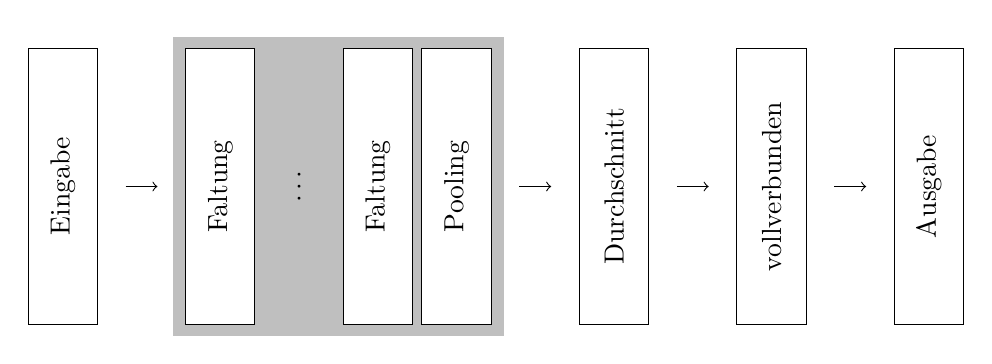
\begin{tikzpicture}[->, shorten >= 10pt, shorten <= 10pt]
  \tikzstyle{node}=[rectangle,draw, minimum width=100pt, minimum height=25pt, inner sep=0pt, fill=white, rotate=90]
  \tikzstyle{noborder}=[draw=none,fill=none]
  \tikzstyle{color1}=[fill=orange]

  \fill [lightgray] (1.4, -1.9) rectangle (5.6, 1.9) node {};

  \node[node] (0)  at (0, 0) {Eingabe};
  \node[node] (1)  at (2, 0) {Faltung};
  \node[node,noborder] (2)  at (3, 0) {$\ldots$};
  \node[node] (3)  at (4, 0) {Faltung};
  \node[node] (4)  at (5, 0) {Pooling};
  \node[node] (5)  at (7, 0) {Durchschnitt};
  \node[node] (6)  at (9, 0) {vollverbunden};
  \node[node] (7)  at (11, 0) {Ausgabe};

  \path (0) edge (1);
  \path (4) edge (5);
  \path (5) edge (6);
  \path (6) edge (7);
\end{tikzpicture}
\caption[Spektrale Netzarchitektur auf Graphen]{Typische spektrale Netzarchitektur auf Graphen bestehend aus beliebig vielen verketteten Faltungsschichten gefolgt von jeweils einer Poolingschicht.
Im Anschluss sorgt die Benutzung einer Durchschnittsschicht über den Knoten jedes Merkmals für die Verwendung von vollverbundenen Schichten hinzu zur Ausgabe.}
\label{fig:netzarchitektur_spectal}
\end{figure}

Alternative Architekturen, auch im Hinblick auf Ersetzungsmöglichkeiten des Average-Poolings, werden in Kapitel~\ref{ausblick} diskutiert.
